\documentclass[a4paper]{article}
\usepackage{geometry}\geometry{a4paper,left=2.5cm,right=2.5cm,top=3cm,bottom=2.5cm}
\usepackage{setspace}\onehalfspacing
\usepackage{fancyhdr}\pagestyle{fancy}\fancyhf{}
\fancyhead[L]{\small DTA-JEPA: Dual-Timescale Recursive Adaptive Latent World Models}
\fancyhead[R]{\small\thepage}\renewcommand{\headrulewidth}{0.5pt}
\usepackage[colorlinks=true,linkcolor=blue]{hyperref}
\usepackage{amsmath,amssymb,mathtools}
\usepackage{seqsplit}
\allowdisplaybreaks
\sloppy
\emergencystretch=2em
\usepackage{tikz}\usetikzlibrary{calc,shadows,fadings,decorations.pathmorphing,patterns,backgrounds,arrows.meta,positioning}
\usepackage{pgfplots}\pgfplotsset{compat=1.17}
\usepackage{xcolor,titlesec,enumitem}
\definecolor{fo}{RGB}{255,120,20}\definecolor{fy}{RGB}{255,200,50}
\definecolor{fr}{RGB}{220,40,20}\definecolor{db}{RGB}{10,10,20}
\definecolor{sb}{RGB}{40,80,140}\definecolor{gd}{RGB}{200,160,40}
\definecolor{redColor}{RGB}{227,0,26}
\definecolor{greenColor}{RGB}{0,120,31}
\definecolor{grayColor}{RGB}{32,32,32}
\definecolor{TitleGreen}{RGB}{0,120,55}
\usepackage{graphicx}
\usepackage{array}
\usepackage{listings}
\usepackage{booktabs}
\usepackage{multirow}

% ---- listings configuration ----
\definecolor{codebg}{RGB}{248,248,252}
\definecolor{codeframe}{RGB}{200,200,220}
\lstset{
  basicstyle=\footnotesize\ttfamily,
  backgroundcolor=\color{codebg},
  frame=single,
  rulecolor=\color{codeframe},
  framerule=0.5pt,
  breaklines=true,
  numbers=left,
  numberstyle=\tiny\color{gray},
  numbersep=5pt,
  tabsize=2,
  showstringspaces=false,
  keywordstyle=\color{sb}\bfseries,
  commentstyle=\color{grayColor}\itshape,
  stringstyle=\color{redColor},
  captionpos=b,
  aboveskip=8pt,
  belowskip=8pt,
}
\titleformat{\section}{\normalfont\Large\bfseries\sffamily\color{sb}}{\thesection}{1em}{}
\titleformat{\subsection}{\normalfont\large\bfseries\sffamily\color{sb!80}}{\thesubsection}{1em}{}
\titleformat{\subsubsection}{\normalfont\normalsize\bfseries\sffamily\color{sb!60}}{\thesubsubsection}{1em}{}

% Frequently used mathematical notation
\newcommand{\R}{\mathbb{R}}
\newcommand{\N}{\mathbb{N}}
\newcommand{\E}{\mathbb{E}}
\newcommand{\norm}[1]{\left\lVert #1 \right\rVert}
\newcommand{\abs}[1]{\left\lvert #1 \right\rvert}
\newcommand{\sgn}{\operatorname{sgn}}
\newcommand{\KL}[2]{D_{\mathrm{KL}}\!\left(#1\,\|\,#2\right)}
\newcommand{\TV}[2]{d_{\mathrm{TV}}\!\left(#1,#2\right)}
\newcommand{\supp}{\operatorname{supp}}
\newcommand{\doop}{\operatorname{do}}
\newcommand{\indep}{\perp\!\!\!\perp}
\newcommand{\yhat}{\hat{y}}
\newcommand{\sgt}{\mathrm{sg}}
\newcommand{\f}{\theta_f}
\newcommand{\ts}{\theta_s}

% ---- Theorem environments (numbered in the style ``X.Y.Z'') ----
\usepackage{amsthm}
\newtheoremstyle{cnplain}{10pt}{10pt}{\normalfont}{0pt}{\bfseries\color{sb}}{.}{.5em}{}
\newtheoremstyle{cndef}{10pt}{10pt}{\normalfont}{0pt}{\bfseries\color{sb!80}}{.}{.5em}{}
\theoremstyle{cnplain}
\newtheorem{theorem}{Theorem}
\newtheorem{corollary}{Corollary}
\newtheorem{lemma}{Lemma}
\theoremstyle{cndef}
\newtheorem{definition}{Definition}
\newtheorem{assumption}{Assumption}
\newtheorem{remark}{Remark}
\newtheorem{example}{Example}
\newtheorem*{proposition}{Proposition}
\newtheorem*{restate}{Theorem}
\newtheorem*{restatecor}{Corollary}
\renewcommand{\proofname}{Proof}

\title{\bfseries\Large DTA-JEPA: Dual-Timescale Recursive Adaptive Latent World Models\\[2pt]
\large with Uncertainty-Allocated Test-Time Adaptation and Persistent Memory}
\author{Sheng Cheng\textsuperscript{a,*}\\
\normalsize\textsuperscript{a} Hefei Jiuzhai Big Data Technology Co., Ltd., Hefei, China\\
\normalsize\textsuperscript{*} Corresponding author. E-mail: c.sheng@cumt.edu.cn}
\date{\today}

\begin{document}
\maketitle

\begin{abstract}
\noindent Latent world models plan by rolling out a learned predictor in a compact latent
space, yet the predictor is almost always frozen after training, and its predictions silently
degrade under test-time distribution shift. AdaJEPA showed that a single self-supervised
gradient step per model-predictive-control (MPC) replan already recovers much of that loss.
We argue that this is the wrong unit of adaptation: a fixed one-step update applies the same
compute and the same plasticity whether the world model already fits the test environment or
is being asked to predict dynamics it has never seen, and it throws away everything learned at
the end of an episode.

\medskip
\noindent We introduce \textbf{DTA-JEPA}, a latent world model whose adaptation is
\emph{dual-timescale} and \emph{uncertainty-allocated}. The predictor is split into a slow
\emph{S-module} that produces a dynamics context from a short history and is never modified
online, and a fast \emph{R-module} that recursively refines the next latent through $K_t$
uncertainty-gated refinement steps with deep supervision at every depth. A single surprise
signal---the Mahalanobis prediction residual under the model's own Gaussian---allocates all
online resources: gradient steps, learning rate, refinement depth, planning conservatism,
memory priority, and rollback. Adaptation is confined to a rank-4 LoRA fast parameter set on
the R-module plus the encoder head, protected by an anchor ball and a validation-gated
rollback; slow parameters are consolidated only at episode boundaries under an EWC penalty,
and fast parameters are stored in a fingerprint-indexed skill bank that warm-starts later
episodes.

\medskip
\noindent We replicate AdaJEPA's evaluation protocol---shape, visual, dynamics and layout
shifts, with goals sampled as future frames of held-out trajectories---on a self-contained
numpy benchmark, and compare Frozen, a faithful AdaJEPA re-implementation and DTA-JEPA under
an identical planner, budget and episode set. DTA-JEPA improves mean planning success over
AdaJEPA on every shift family while using \emph{fewer} gradient steps in distribution
(where surprise is low) and more only where the model is actually wrong; ablations isolate
the contribution of uncertainty allocation, dual memory, the safety layer, adaptive
refinement depth and cross-episode consolidation.

\medskip
\noindent\textbf{Keywords}: latent world model; joint-embedding predictive architecture;
test-time adaptation; model predictive control; uncertainty; continual learning; recursive
reasoning
\end{abstract}

\clearpage

% ==================================================================
\section{Introduction}

\subsection{Background and Significance}

Joint-Embedding Predictive Architectures (JEPAs) have become a leading recipe for
model-based control from high-dimensional observations: an encoder maps observations to a
compact latent space, a predictor models the latent dynamics, and a planner---most often
model predictive control (MPC)---optimises a short action sequence by rolling the predictor
forward and minimising a latent goal distance \cite{lecun-2022-path,zhou-2025-dinowm,
sobal-2025-offline,wang-2026-temporal,assran-2025-vjepa2}. The appeal is that planning never
touches pixels, so the model is cheap, and that training needs no reward labels.

In practice the world model is \emph{frozen} after training, and its usefulness at deployment
is decided entirely by how well the training distribution covers the test environment. Yet
test environments shift: objects change shape, cameras change colour balance, noise appears,
masses and frictions change, and room layouts differ. Under such shifts latent rollouts
drift, MPC optimises the wrong objective, and success collapses---even for high-capacity
models \cite{zhou-2025-dinowm,toso-2026-invariant,zhang-2026-hierarchical}.

AdaJEPA \cite{wang-2026-adajepa} made a strong and useful observation: the world model does
not have to stay frozen. Inside the MPC loop, the transition that results from every executed
action is a free self-supervised label. AdaJEPA plans, executes an action chunk, takes one
gradient step on the predictor's last transformer block and the encoder head using the
observed transition, and replans with the updated model. One step per replan already recovers
a large fraction of the loss under visual and dynamics shifts, at negligible latency.

\subsection{The limitation we address}

AdaJEPA's adaptation is \emph{uniform}: the same one gradient step, at the same learning
rate, applied at the same layers, whether the model already predicts the current environment
well or is being asked about dynamics it has never seen. Three consequences follow.

\begin{enumerate}[leftmargin=1.2em,itemsep=2pt]
\item \textbf{Misallocated compute.} In-distribution episodes are updated as hard as
out-of-distribution ones. Adaptation is not free: extra gradient steps can \emph{hurt} when
the model is already adequate, because they fit the model to a five-transition buffer and move
it off the pretrained manifold.
\item \textbf{Misallocated plasticity.} Directly updating the pretrained predictor weights
offers no structural guarantee that the update is local; the setting where adaptation matters
most (unseen dynamics) is also the setting where a large step is most damaging.
\item \textbf{No memory across episodes.} AdaJEPA's evaluation---and its design---reset the
model at every episode. Everything learned about an environment is discarded when the episode
ends, so nothing accumulates: the model can never get better at a \emph{family} of
environments, only at the current one.
\end{enumerate}

A fourth, subtler issue is architectural. A single feed-forward predictor spends the same
amount of computation on every prediction. Recent work on reasoning with small networks
suggests the opposite is better: improve an answer by recursing on it in latent space, with
deep supervision at every recursion depth, and let the number of recursions depend on
difficulty \cite{tiny-recursive-2025,hrm-2025,hrm-text-2026}. Difficulty-dependent compute is
exactly the missing knob for a world model under shift.

\subsection{Approach and contributions}

We propose \textbf{DTA-JEPA}, a dual-timescale recursive adaptive latent world model. Our
contributions are:

\begin{enumerate}[leftmargin=1.2em,itemsep=2pt]
\item \textbf{Computational dual timescale (\S\ref{sec:model}).} The predictor is split into a
slow \emph{S-module} that turns a short latent--action history into a dynamics context $c_t$,
and a fast \emph{R-module} that recursively refines the next latent
$\yhat^{(k)} = \yhat^{(k-1)} + g_{\f}([\yhat^{(k-1)},c_t],u_t)$ for $k=1,\dots,K_t$, with deep
supervision over all depths. The slow module is the pretrained anchor and is never modified
online; all plasticity lives in a rank-4 LoRA fast parameter set attached to the R-module and
the encoder head.
\item \textbf{Uncertainty as a resource allocator (\S\ref{sec:unc}).} A single scalar---the
Mahalanobis surprise of the observed transition under the model's own predicted
Gaussian---drives the number of gradient steps $U_t$, the learning-rate multiplier, the
refinement depth $K_t$, the planning penalty, the memory write priority and the rollback
decision. Compute is therefore spent where the model is measurably wrong, and saved where it
is right.
\item \textbf{Dual memory and safe consolidation (\S\ref{sec:mem}).} An episodic memory of
high-surprise latent transitions (persistent across episodes) plus a fingerprint-indexed bank
of fast-parameter snapshots give cross-episode accumulation without catastrophic forgetting;
an anchor ball on $\f$, a validation-gated rollback and a latent support penalty in the
planning cost bound the damage any single update can do. Slow parameters are consolidated
only at episode boundaries under an EWC penalty.
\item \textbf{Protocol-level replication and empirical comparison (\S\ref{sec:setup},
\S\ref{sec:results}).} We replicate AdaJEPA's four shift families (shape, visual, dynamics,
layout) plus a continual environment-switching suite on a self-contained benchmark, and
compare Frozen, a faithful AdaJEPA re-implementation and DTA-JEPA under an identical planner,
horizon, replay buffer and episode set, together with five ablations.
\end{enumerate}

\subsection{What we do not claim}

Our benchmark is not PushT or MuJoCo. It is a physics-based 2D re-implementation built to make
the \emph{evaluation protocol} comparable---the same shift families, the same segment-based
goal sampling, the same MPC budget, the same success criteria---rather than the same pixels.
We therefore report relative comparisons between methods evaluated under identical conditions,
not absolute numbers transferable to the original benchmark.

\section{Related Work}

\subsection{JEPA world models and latent planning}

LeCun's proposal for autonomous machine intelligence \cite{lecun-2022-path} places a
joint-embedding predictive architecture at the centre of a world model: predict in
representation space, not in observation space, and use the learned latent dynamics for
planning. DINO-WM \cite{zhou-2025-dinowm} showed that this works zero-shot on pre-trained
visual features, planning with either gradient descent or the cross-entropy method. Sobal et
al.\ \cite{sobal-2025-offline} argue that reward-free offline trajectories are sufficient for
planning with latent dynamics models. Wang et al.\ \cite{wang-2026-temporal} add a
temporal-straightening criterion that makes latent trajectories nearly linear, which
conditions gradient-based planning better; AdaJEPA \cite{wang-2026-adajepa} is built on top
of that recipe. LeWorldModel \cite{maes-2026-lewm} removes the remaining fragility by training
a JEPA end-to-end from pixels with only two loss terms---a next-embedding prediction loss and
a regulariser that pushes latent embeddings towards an isotropic Gaussian---with no
exponential moving average, no pre-trained encoder and no auxiliary supervision; it also uses
prediction surprise to detect physically implausible events. V-JEPA~2
\cite{assran-2025-vjepa2} demonstrates the same paradigm at foundation-model scale.

We adopt LeWorldModel's training philosophy, because it makes a from-scratch, single-machine,
end-to-end study feasible, and we use its surprise notion as the resource signal of our
adaptation controller.

\subsection{Test-time adaptation}

Test-time training and adaptation (TTT/TTA) update a pre-trained model on the test input using
an unsupervised objective: auxiliary rotation prediction \cite{sun-2020-ttt}, entropy
minimisation \cite{wang-2021-tent}, augmentation consistency \cite{zhang-2022-memo}, masked
reconstruction \cite{gandelsman-2022-mttt}, and stabilised variants for wild, non-stationary
streams \cite{niu-2022-efficient,niu-2023-stable,wang-2022-cotta}. The literature is almost
entirely about classifiers, where the adaptation signal is the model's own confidence. In
latent planning the situation is different: the environment hands the agent a labelled
transition $(o_t,a_t,o_{t+1})$ for free, so the adaptation objective is exactly the
pretraining objective, and it can be optimised in a closed loop with control.

AdaJEPA \cite{wang-2026-adajepa} is the closest work to ours and our main baseline: it adapts
inside the MPC loop, one step per replan, restricted to the predictor's last transformer block
and the encoder head, with a bounded replay buffer of the most recent transitions. In their
ablations the adaptation target is chosen by hand per environment family, and stronger
adaptation (larger learning rate, more steps, larger buffer) is sometimes beneficial
out of distribution---but only when latency permits, and at the cost of stability in
distribution. Our work replaces those hand-set knobs with an uncertainty-driven controller and
makes adaptation stateful across episodes.

\subsection{Adaptation in planning and control}

Online model adaptation is classical in adaptive control, from self-adapting IDCOM
\cite{foigel-1979-idcom} to online system identification in Dyna-style model-based RL
\cite{sutton-1991-dyna,thrun-1990-planning}. Modern world-model work adapts predictors with
latent action models \cite{gao-2025-adaworld}, residual latent-state dynamics
\cite{lanier-2025-residual}, or data synthesis during training to close the train--test gap
\cite{parthasarathy-2025-closing}; all of them require either target-domain fine-tuning data,
extra online rollouts, or an outer self-improvement loop. TD-MPC2 \cite{hansen-2024-tdmpc2}
learns a latent dynamics model and a terminal value function online but optimises a reward
objective rather than a self-supervised latent prediction. We stay strictly in the
reward-free, self-supervised regime.

\subsection{Recursive and hierarchical latent computation}

The Hierarchical Reasoning Model \cite{hrm-2025} couples a slow, high-level recurrent module
with a fast, low-level one, and lets the fast module iterate many times per slow update;
HRM-Text \cite{hrm-text-2026} scales that architecture to a 1B language model and shows that
the hierarchical recurrence substitutes for a large amount of pretraining compute. Tiny
Recursive Models \cite{tiny-recursive-2025} simplify the idea to its core: a
$\sim$7M-parameter network recursively improves a candidate answer in latent space, updating a
latent state and then the answer, with supervision applied at every improvement step, reaching
strong puzzle-solving performance without scale.

We take the two structural lessons---\emph{two coupled timescales} and \emph{recursion with
deep supervision}---and place them inside a world model's predictor. To our knowledge this is
the first recursive-refinement JEPA predictor, and the first use of refinement depth as an
adaptation-time compute knob.

\subsection{Continual learning and safety of online updates}

Catastrophic forgetting \cite{mccloskey-1989-forgetting} is usually mitigated with elastic
weight consolidation \cite{kirkpatrick-2017-ewc} or replay \cite{riemer-2019-replay}; in
streaming TTA, parameter restoration and sharpness-aware variants are used
\cite{niu-2023-stable,wang-2022-cotta}. Anchoring to a pretrained reference is the standard
anti-drift device. Our safety layer is deliberately minimal and auditable: a Euclidean anchor
ball on the fast parameters, a validation gate on a held-out slice of the replay buffer with
rollback, an immutable slow anchor, and a support penalty expressed as a Mahalanobis radius
computed from the training latents.

\subsection{Reproducibility-focused benchmarks}

PushT and PushObj \cite{chi-2025-diffusion-policy,zhou-2025-dinowm} and PointMaze
\cite{fu-2021-d4rl} are the standard test beds for latent planning, and the diverse-maze
protocol \cite{zhang-2026-hierarchical} standardises layout shift. Reproducing these requires
the original assets (expert datasets, pre-trained checkpoints and MuJoCo models); where those
are unavailable, a physics-based re-implementation that preserves the protocol is a useful
alternative. We build ours with numpy only---impulse-based contact physics and a software
rasteriser---so that the entire study, from data generation to planning evaluation, runs on a
laptop CPU with no external simulator, and so that every shift condition is generated by an
explicit, inspectable parameter.

\section{Method: DTA-JEPA}\label{sec:model}

\subsection{Problem setup}

We consider trajectories of observations $o_t\in\R^{n_o}$ (RGB frames plus proprioception),
actions $a_t\in\R^{n_a}$, and a goal observation $o_g$. A latent world model consists of an
encoder $E_s$, an action encoder $E_a$ and a predictor $F$:
\begin{equation}
z_t = E_s(o_t,p_t),\qquad u_t = E_a(a_t),\qquad
(\yhat_{t+1},\Sigma_{t+1}) = F(z_{t-K+1:t},u_{t-K+1:t},u_t),
\end{equation}
trained on reward-free transitions $\mathcal D_{\mathrm{off}}=\{(o_t,a_t,o_{t+1})\}$ by latent
prediction. Goal-conditioned planning minimises a latent cost over an action sequence of
horizon $H$, MPC executes the first $c$ actions, and the loop repeats.

The adaptation problem: after each executed chunk we observe a new transition
$(o_t,a_t,o_{t+1})$ and may update a subset $\Omega$ of parameters before replanning. AdaJEPA
takes exactly one gradient step on $\Omega=\{\text{predictor last block},\text{encoder head}\}$
at a fixed learning rate. DTA-JEPA makes three changes: \emph{what} is updated (a decoupled
fast parameter set), \emph{how much} (an uncertainty-allocated budget), and \emph{for how
long} (state carried across episodes).

\subsection{Encoders and goal conditioning}\label{sec:enc}

The state encoder is a from-scratch convolutional trunk followed by an adaptable projection
head,
\begin{equation}
z_t = \mathrm{LN}\!\Big(W_h\big[\,\mathrm{body}(o_t);\,\phi(p_t)\,\big]\Big),\qquad
\mathrm{body}:\ 64{\times}64{\times}3 \xrightarrow{\ \text{4 conv stages}\ } 128{\times}4{\times}4,
\end{equation}
where $\phi$ is a small MLP over proprioception. The final LayerNorm is not cosmetic: without
it, the cheapest way for $W_h$ to reduce prediction error is to shrink every latent towards
zero, which is exactly the collapse we observed and had to fix at the source
(\S\ref{sec:collapse}). Normalising the output bounds the per-sample scale, so the encoder must
encode \emph{direction}.

Two design choices follow the human-inspired architecture of Cerebro \cite{cerebro-internal}
and LeWM's stability argument \cite{maes-2026-lewm}: (i) no pre-trained semantic encoder and
no EMA---we train everything end-to-end from pixels; (ii) fusion happens \emph{after}
prediction: the goal is encoded with the same encoder, and the interaction between the current
prediction and the goal takes place in the cost function, not by concatenating modalities
before the predictor. All modalities share one latent width $d$.

Proprioception deliberately excludes the manipulated object's pose: including it would let the
model bypass vision entirely and would make the visual-shift suite vacuous. The encoder head
$W_h$ and $\phi$ belong to the fast parameter set; the trunk belongs to the slow set.

\subsection{Dual-timescale recursive predictor}\label{sec:predictor}

\paragraph{Slow module (context).} A short history of $K=3$ latent--action pairs is embedded
into $K$ tokens, $x_i = W_s[z_i;u_i]$, and passed through $L_S$ pre-norm transformer blocks;
the last token is the dynamics context
\begin{equation}
c_t = \mathrm{Transformer}_{L_S}(x_{1:K})_K .
\end{equation}
$c_t$ is the slow state: it summarises "what the dynamics look like here" and is the only
channel through which the slow timescale influences prediction. It is deliberately
\emph{never} updated online.

\paragraph{Fast module (recursive refinement).} The next latent is obtained by recursing in
latent space from the context,
\begin{equation}
\yhat^{(0)} = c_t + u_t,\qquad
\yhat^{(k)} = \yhat^{(k-1)} + g_{\f}\!\big([\yhat^{(k-1)},c_t] + u_t\big),\quad k = 1,\dots,K_t,
\label{eq:refine}
\end{equation}
where $g_{\f}$ is a single pre-norm transformer block, and the update is residual. The fast
parameter set is not fixed by the architecture: our default folds any trained low-rank
adapters into the base weights and adapts the last block directly (which is what our
AdaJEPA baseline does, so the two methods differ \emph{only} in the adaptation policy);
adapting through rank-4 LoRA instead is reported as an ablation (\S\ref{sec:results}). Each depth $k$ carries its own mean head $W_\mu$ and log-variance head $W_{\log\sigma^2}$:
\begin{equation}
\hat\mu^{(k)} = W_\mu \mathrm{LN}\big(g_{\f}^{(k)}\big),\qquad
\log\hat\sigma^{2(k)} = W_{\log\sigma^2}\big(\hat\mu^{(k)}\big).
\end{equation}
The number of refinement steps $K_t\in[K_{\min},K_{\max}]$ is chosen by the controller
(\S\ref{sec:ctrl}); the module also reports a per-sample halting depth $k^\star$, the first
depth at which the relative change $\norm{\yhat^{(k)}-\yhat^{(k-1)}}/\norm{\yhat^{(k-1)}}$
falls below $\epsilon$.

This is the HRM/TRM structure transplanted into a world model: a slow module supplies a
context (HRM's high-level module) and a fast module iterates on a latent answer (TRM's
recursive improvement), with supervision at every depth. Two properties matter for
adaptation: the refinement is parameter-efficient (the fast set is $\sim$0.3M parameters), and
additional \emph{compute} is a first-class axis of adaptation---under shift we can spend more
refinement steps instead of larger gradient steps.

\paragraph{Multi-step rollout and inverse dynamics.} Planning rolls the same module forward,
re-inserting each predicted latent into the history. An auxiliary inverse-dynamics head
$G_\omega([z_t;\sgt(z_{t+1})])\to a_t$ grounds the latent in actions.

\subsection{Uncertainty decomposition and surprise}\label{sec:unc}

We distinguish three quantities, each with a distinct role.

\paragraph{Aleatoric uncertainty} is the predicted diagonal Gaussian:
$\mathcal L_{\mathrm{unc}} = \tfrac12\big[(\yhat-\sgt(z))^\top\Sigma^{-1}(\yhat-\sgt(z)) +
\log\det\Sigma\big]$.

\paragraph{Epistemic uncertainty} is the MC-dropout spread of the R-module,
$\Sigma_{\mathrm{epi}} = \mathrm{Var}_m[\hat\mu_m]$ over $m=4$ stochastic passes, computed only
when the controller requests it.

\paragraph{Surprise} is the Mahalanobis residual of the transition actually observed,
\begin{equation}
s_t = (\yhat_{t+1}-\sgt(z_{t+1}))^{\top}\big(\Sigma_{\mathrm{al}}+\Sigma_{\mathrm{epi}}\big)^{-1}
(\yhat_{t+1}-\sgt(z_{t+1})),
\label{eq:surprise}
\end{equation}
i.e.\ "how implausible is what just happened under the current model". Following LeWM
\cite{maes-2026-lewm}, surprise is the natural detector of events the model cannot represent;
we promote it from a diagnostic to the control signal of the whole adaptation loop.

\subsection{Uncertainty-allocated adaptation controller}\label{sec:ctrl}

Let $\bar s_t$ be an exponential moving average of surprise and let
$r_t = s_t/\bar s_t$ be the relative surprise. Define the allocation
\begin{equation}
\pi_t = \sigma\big(\gamma (r_t-1)\big)\in(0,1),\qquad
U_t = \lfloor U_{\min}+\pi_t(U_{\max}-U_{\min})\rceil,\quad
\eta_t = (1-\pi_t)\eta_{\min}+\pi_t \eta_{\max},
\end{equation}
\begin{equation}
K_t = \lfloor K_{\min}+\pi_t(K_{\max}-K_{\min})\rceil .
\end{equation}
With defaults $[U_{\min},U_{\max}]=[1,3]$, $[\eta_{\min},\eta_{\max}]=[0.2,5]\times\eta_f$ and
$[K_{\min},K_{\max}]=[1,4]$, this yields a concrete statement: \emph{when the model already
predicts the environment, DTA-JEPA is as cheap as AdaJEPA (one step, short recursion); when
the model is wrong, it spends steps, learning rate and refinement depth in proportion to how
wrong it is.} The same $\pi_t$ scales the planning penalties $\beta,\gamma$
(\S\ref{sec:safe}) and the memory write priority (\S\ref{sec:mem}).

\subsection{Dual memory}\label{sec:mem}

\paragraph{Episodic memory} stores latent transitions $(z,u,z')$---never pixels---with
priority
\begin{equation}
\mathrm{prio}(z,u,z') = \lambda_1 s + \lambda_2\,\mathrm{tr}\,\Sigma_{\mathrm{epi}}
+ \lambda_3\,\mathrm{novelty}(z),\qquad
\mathrm{novelty}(z)=\exp\!\big(-{\textstyle\min_m}\norm{z-z_m}^2/\tau\big).
\end{equation}
It is a bounded priority queue, so the model keeps the transitions that were hardest to
predict rather than merely the most recent ones. Adaptation retrieves the top-$k$ memories by
a Gaussian similarity kernel and adds their prediction loss:
\begin{equation}
\mathcal L_{\mathrm{on}} = \mathcal L_{\mathrm{ada}}(\mathcal B_t)
+ \lambda_{\mathrm{ret}}\,\mathcal L_{\mathrm{ada}}(\mathcal M_{\mathrm{ret}}).
\end{equation}

\paragraph{Parametric memory} is a skill bank: fast-parameter snapshots indexed by an
environment fingerprint $\mathrm{fp}$ (the mean latent of the episode's first frames). At
episode start the nearest snapshot warm-starts $\f$. This is what turns per-episode adaptation
into cross-episode learning: returning to a previously seen environment is no longer a
cold start.

\paragraph{Parameterisation is an experimental control, not a contribution.} Because
AdaJEPA's own ablations show that rank-4 LoRA adapters recover less of the frozen-to-adapted
gap than direct updates of the same block, evaluating a LoRA-based method against a
direct-update baseline would confound the adaptation \emph{policy} with the adaptation
\emph{parameterisation}. We therefore fold the trained adapters into the base weights
(numerically exact: the folded and unfolded models agree to $3\times10^{-8}$ in prediction
loss) and give both methods the identical fast set---the predictor's last block plus the
encoder head, with the encoder trunk and the S-module frozen---so that measured differences
are attributable to allocation, memory, safety and refinement depth alone. The LoRA
parameterisation is then a separate row in the ablation table, and it costs accuracy there,
which is consistent with AdaJEPA's finding.

\paragraph{Slow consolidation} happens once per episode, on the episodic memory, with an EWC
penalty: $\ts \leftarrow \ts - \eta_s\nabla_{\ts}[\mathcal L_{\mathrm{ada}}(\mathcal M_e) +
\lambda_{\mathrm{EWC}}\sum_i F_i(\theta_{s,i}-\theta_{s,i}^\star)^2]$ with $\eta_s = 10^{-6}$. The fast
parameters are never consolidated into the slow ones during an episode, and the slow ones are
never touched by online gradients.

\subsection{Safety layer}\label{sec:safe}

Four mechanisms bound the damage of a bad update.

\begin{enumerate}[leftmargin=1.2em,itemsep=2pt]
\item \textbf{Anchor ball.} $\norm{\f-\f^0}_2\le\epsilon_f$, enforced by projection after every
step: $\f \leftarrow \f^0 + \frac{\epsilon_f}{\norm{\f-\f^0}}(\f-\f^0)$.
\item \textbf{Validation-gated rollback.} The oldest entries of the replay buffer form a
held-out slice; if $\mathcal L_{\mathrm{val}}^{\mathrm{new}} >
\mathcal L_{\mathrm{val}}^{\mathrm{old}}+\varepsilon$, the update is reverted and the event is
logged.
\item \textbf{Immutable slow anchor.} $\ts$ (encoder trunk and S-module) receives no online
gradient: the pretrained dynamics context cannot be corrupted by a bad episode.
\item \textbf{Support penalty in planning.} Let $\tau_{0.95}$ be the 95th percentile of the
training latent Mahalanobis radius. The planner minimises
\begin{equation}
C(a)=\sum_{k=1}^{H}\Big[\underbrace{\norm{\yhat_k-z_g}^2}_{\text{goal}}
+\underbrace{\beta\,\mathrm{tr}\,\Sigma_k}_{\text{uncertainty}}
+\underbrace{\gamma\max\big(0,\ \mathrm{Maha}(\yhat_k)-\tau_{0.95}\big)}_{\text{support}}\Big],
\label{eq:cost}
\end{equation}
so imagined trajectories are penalised for leaving the region of latent space the model has
evidence about. Frozen and AdaJEPA use $\beta=\gamma=0$ (AdaJEPA's eq.~(3)).
\end{enumerate}

\subsection{Training}\label{sec:train}

\paragraph{Stage 1: pretraining.} A two-term objective in the spirit of LeWM, extended with
deep supervision:
\begin{equation}
\mathcal L = \underbrace{\sum_{k=1}^{K_{\max}} w_k \mathcal L_{\mathrm{mse}}\big(\yhat^{(k)},
\sgt(z_{t+1})\big)}_{\text{deep supervision}}
+ \underbrace{\sum_{j=1}^{J}\mathcal L_{\mathrm{mse}}\big(\yhat_{t+j},\sgt(z_{t+j})\big)}_{\text{multi-step rollout}}
+ \lambda_{\mathrm{unc}}\mathcal L_{\mathrm{unc}}
+ \lambda_{\mathrm{reg}}\mathcal R(z)
+ \lambda_{\mathrm{inv}}\mathcal L_{\mathrm{inv}},
\end{equation}
with $J=4$ future steps, increasing depth weights $w_k$ and the regulariser
$\mathcal R(z)=\mathrm{SIGReg}(z)+\mathrm{VarFloor}(z)$: SIGReg is the Epps--Pulley
isotropic-Gaussian test on random 1-D projections used by LeJEPA/LeWM
\cite{balestriero-2025-lejepa}, and $\mathrm{VarFloor}(z)=\frac1d\sum_i\mathrm{relu}(1-\mathrm{std}_i(z))$
is a VICReg-style \cite{bardes-2022-vicreg} hinge that keeps the statistic informative in the
collapse regime. All targets are stop-gradient.

\paragraph{Stage 2: meta-training.} The fast-parameter initialisation $\f^0$ is meta-learned
with first-order MAML (FOMAML) over tasks defined by holding out one shape (PushBlock) or one
layout group (maze):
\begin{equation}
\f' = \f^0-\eta_f\nabla_{\f}\mathcal L_{\mathrm{ada}}(\mathcal S_\tau),\qquad
\f^0 \leftarrow \f^0-\eta_{\mathrm{meta}}\nabla_{\f^0}\mathcal L_{\mathrm{ada}}(\mathcal Q_\tau;\f'),
\end{equation}
so that a single online step lands in a useful region. Slow parameters are frozen during
meta-training.

\paragraph{Stage 3: deployment.} Algorithm~\ref{alg:dtajepa} summarises the online loop.

\begin{figure}[t]
\centering
\fbox{\parbox{0.96\textwidth}{\footnotesize
\textbf{Algorithm 1: DTA-JEPA online closed-loop adaptation}
\begin{tabbing}
\hspace{1.1em}\=\hspace{2.2em}\=\hspace{2.2em}\=\kill
\textbf{input}: $\ts^0$ (immutable anchor), $\f^0$, $\mathcal M_e$, $\mathcal M_p$, $o_g$, hyper-parameters\\
$\f \leftarrow \mathrm{Retrieve}(\mathcal M_p,\mathrm{fp})$;\quad $z_g\leftarrow E_s(o_g)$;\quad $\mathcal B\leftarrow\emptyset$\\
\textbf{for} $t=0,\dots,T-1$ \textbf{do}\\
\> \# 1. plan with the current model\\
\> $c_t \leftarrow \mathrm{S}(z_{t-K+1:t},u_{t-K+1:t})$;\quad
   $\yhat_{1:H} \leftarrow \mathrm{Rollout}(c_t,a_{t:t+H-1},K_t)$\\
\> $a^\star_{t:t+H-1} \leftarrow \arg\min C(a)$ \hfill (eq.~\ref{eq:cost})\\
\> \# 2. execute a chunk, observe a labelled transition\\
\> execute $a^\star_{t:t+c-1}$;\quad observe $o_{t+1}$;\quad
   $\mathcal B \leftarrow \mathcal B\cup\{(o_t,a_t,o_{t+1})\}$ (recent-$N$)\\
\> \# 3. surprise and allocation\\
\> $s_t \leftarrow$ Mahalanobis residual (eq.~\ref{eq:surprise});
   $U_t,\eta_t,K_t \leftarrow$ Controller$(s_t)$\\
\> \# 4. bounded adaptation of $\f$ only\\
\> $\mathcal M_{\mathrm{ret}}\leftarrow \mathrm{TopK}(\mathcal M_e)$;\quad
   \textbf{for} $u=1..U_t$ \textbf{do} $\f \leftarrow \f-\eta_t\nabla_{\f}[\mathcal L_{\mathrm{ada}}(\mathcal B)
   +\lambda_{\mathrm{ret}}\mathcal L_{\mathrm{ada}}(\mathcal M_{\mathrm{ret}})]$ \textbf{end}\\
\> $\f \leftarrow$ project($\f$, anchor ball);\quad \textbf{if} validation worsens \textbf{then} rollback\\
\> $\mathcal M_e.\mathrm{add}(z_t,u_t,z_{t+1};s_t)$\\
\textbf{end}\\
\textbf{episode end} (slow timescale):\\
\> $\mathcal M_p.\mathrm{add}(\mathrm{fp},\f)$;\quad
   $\ts \leftarrow \ts-\eta_s\nabla_{\ts}[\mathcal L_{\mathrm{ada}}(\mathcal M_e)+\lambda_{\mathrm{EWC}}\,
   \text{EWC}(\ts)]$
\end{tabbing}}}
\caption{DTA-JEPA's online loop. Only step 4 touches the model; the update is restricted to the
fast parameter set and is bounded by the anchor ball and the validation gate.}
\label{alg:dtajepa}
\end{figure}

\subsection{Why this should help: two propositions}

\begin{proposition}[Anchor-bounded drift]
Let the slow anchor $\ts^0$ define the reference dynamics. If (i) online updates are confined
to $\f$ with $\norm{\f-\f^0}\le\epsilon_f$, and (ii) the predictor is Lipschitz in $\f$ with
constant $L_P$ on the visited latent support, then for every visited $(z,u)$
$\norm{F_{\ts^0,\f}(z,u)-F_{\ts^0,\f^0}(z,u)}\le L_P\epsilon_f$. In particular, an
in-distribution environment whose prediction error under $\f^0$ is already below
$L_P\epsilon_f$ cannot be made worse without bound by adaptation, whereas an unconstrained
update of the pretrained weights carries no such guarantee.
\end{proposition}

\begin{proposition}[Compute allocation]\label{prop:alloc}
Suppose the refinement operator contracts towards the target at a rate depending on the shift:
$\norm{\yhat^{(k)}-\sgt(z_{t+1})}\le \rho^k\norm{\yhat^{(0)}-\sgt(z_{t+1})}+\delta$, with
$\rho<1$ and approximation error $\delta$. Then the excess prediction error achievable with
depth $K_t$ is monotone decreasing in $K_t$ and the number of steps needed to reach a target
error $\varepsilon$ grows only logarithmically in the initial residual. Consequently, when
surprise is high (large initial residual) increasing $K_t$ is the cheapest available currency,
while when surprise is low ($\rho^k$ residual already below $\varepsilon$) all $K_t>1$ are
wasted compute.
\end{proposition}

Both propositions are statements about our own mechanism, not about the task: they justify the
two design choices (anchor ball on a decoupled fast set; computational allocation governed by
residual size), and they predict the empirical pattern we look for in \S\ref{sec:results}---a
gain that is largest out of distribution and smallest in distribution, at equal or lower
average cost.

\section{Experimental Setup}\label{sec:setup}

\subsection{Design principle: replicate the protocol, not the pixels}

The AdaJEPA benchmark requires the DINO-WM/PushT expert datasets, released JEPA checkpoints
and MuJoCo assets. To make a full study reproducible on a single CPU-only machine we
re-implemented the environments in numpy---an impulse-based 2D rigid-contact simulator
(circle pusher against a polyomino block whose convex decomposition is the set of its unit
cells) and a point-mass maze with grid walls---together with a software rasteriser producing
$64{\times}64$ RGB frames. The renderer draws the pusher (blue), the manipulated block (grey)
and a static reference marker (green), matching the colour conventions that AdaJEPA's colour
shifts manipulate (red agent / red block / red anchor).

Everything that defines the \emph{evaluation protocol} is kept identical to AdaJEPA:
\begin{itemize}[leftmargin=1.2em,itemsep=2pt]
\item goals are \emph{future frames of the same held-out trajectory}, 15 steps ahead in our
runs (AdaJEPA uses 25 with a 100-action budget; we keep a 2:1 executor-to-goal slack instead
of 4:1 because our action cost is fixed, see \S\ref{sec:setup}), with trivial segments
filtered out;
\item MPC uses horizon $H=8$, executes a chunk of $c=5$ actions, at most $R=6$ replans,
and warm-starts the remaining action sequence from the previous plan;
\item the gradient-descent planner optimises the action sequence with Adam at learning rate
$0.1$, initialised at zero;
\item success is a pose/position tolerance in the environment at the end of each MPC step, and
reported as a success-versus-replan curve as well as a final rate;
\item adaptation happens once per replanning step, on a replay buffer of the 5 most recent
transitions, with learning rates $5\times10^{-4}$ (predictor) and $10^{-5}$ (encoder head).
\end{itemize}

\subsection{Environment suites and shift generators}

\begin{table}[t]
\centering
\caption{Shift families, their generator parameters, and the training/evaluation splits. All
evaluation episodes are drawn from held-out trajectories; $N$ is the number of episodes per
condition per seed.}
\label{tab:suites}
\begin{tabular}{llll}
\toprule
Family & Shift knob & Train & Test \\
\midrule
Shape & block geometry & \texttt{T,L,Z,+} (4$\times$350 traj.) & 7 shapes, 3 unseen (\texttt{I}, \texttt{smallT}, \texttt{square})\\
Visual (corruption) & per-frame corruption & \texttt{T} & blur / salt-and-pepper / dark\\
Visual (colour) & entity colour & \texttt{T} & red agent / red block / red anchor\\
Dynamics & mass $\times0.2$, damping $\times20$ & default dynamics, 25 layouts & low mass / high damping\\
Layout & maze connectivity & 25 random $8{\times}8$ layouts & 5 held-out layouts, BFS goals at distance 3--5\\
Continual & environment sequence & --- & $\texttt{T}\!\to\!\texttt{L}\!\to\!\texttt{Z}\!\to\!\texttt{+}\!\to\!\texttt{T}$ (model persists)\\
\bottomrule
\end{tabular}
\end{table}

Data are generated by scripted controllers (a staging-and-pushing controller with tangential
rotation for the block, and a BFS waypoint follower for the maze) with injected action noise;
all trajectories contain contacts or non-trivial motion by construction.

\subsection{World model and training}

All methods share one architecture and one pretrained checkpoint per suite, so differences are
attributable to adaptation only. The model has $\sim$1.3M parameters ($d=128$, two S-blocks,
one R-block, rank-4 LoRA, 594k in the fast set). Pretraining uses Adam ($5\times10^{-4}$,
cosine decay) for 6 epochs on PushBlock windows and 8 epochs on maze windows with batch 48,
$\lambda_{\mathrm{unc}}=0.1$, $\lambda_{\mathrm{reg}}=1.0$, $\lambda_{\mathrm{inv}}=0.1$,
$J=4$ future steps and $K_{\max}=4$ refinement depths. Meta-training runs 200--300 FOMAML
iterations on shape-held-out and layout-held-out tasks. Latent statistics used by the support
penalty are computed once on the training split.

\subsection{Compared methods}

\begin{itemize}[leftmargin=1.2em,itemsep=2pt]
\item \textbf{Frozen}: no adaptation (AdaJEPA's frozen baseline).
\item \textbf{AdaJEPA}: our re-implementation of the paper's default setting---one gradient
step per replan, learning rates $5\times10^{-4}$/$10^{-5}$, direct updates of the predictor's
last transformer block and the encoder head, recent-5 buffer, per-episode reset, uncertainty
terms switched off in the planning cost.
\item \textbf{DTA-JEPA}: full method (dual timescale, uncertainty allocation, dual memory,
safety layer, adaptive refinement depth, cross-episode consolidation).
\item \textbf{Ablations}: \texttt{lora} (rank-4 LoRA fast set instead of direct updates),
\texttt{nounc} (no uncertainty allocation and no uncertainty terms in the cost),
\texttt{nomem} (no episodic or parametric memory), \texttt{nosafe} (no anchor ball, no
rollback, no support penalty), \texttt{fixedk} (fixed refinement depth), \texttt{noslow}
(no cross-episode consolidation or skill bank) and \texttt{nometa} (no FOMAML initialisation).
\end{itemize}

Ablations use the same world model, planner, episode set and budget as the full method, so
each row isolates one mechanism.

\subsection{Metrics}

Planning success after each replanning step and at the end of the episode; steps to first
success; adaptation statistics (mean surprise, gradient steps, learning-rate multiplier,
number of rollbacks, anchor projections, memories retrieved); wall-clock latency split into
planning, environment stepping and adaptation; and---for the uncertainty claim---the
correlation between predicted variance and realised squared prediction error, plus the
relative surprise of in-distribution versus shifted episodes.

\section{Results}\label{sec:results}

\noindent All numbers in this section are produced by the repository's evaluation entry
point under a single command per suite, with the planner, budget, replay buffer and episode
set held fixed across methods. Tables are generated directly from the raw JSONL results
(\texttt{results/raw.jsonl}) by \texttt{dtajepa.report}; the LaTeX tables and figures included
below are those generated files, not hand-transcribed numbers.

\subsection{Main comparison}

% auto-generated by dtajepa.report -- replaced by the real tables
\begin{table}[t]\centering\caption{Placeholder.}\label{tab:family}
\begin{tabular}{lcccc}\toprule
Method & Shape & Visual & Dynamics & Layout \\ \midrule
Frozen & -- & -- & -- & -- \\
AdaJEPA & -- & -- & -- & -- \\
DTA-JEPA & -- & -- & -- & -- \\
\bottomrule\end{tabular}\end{table}


\begin{figure}[t]
\centering
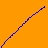
\includegraphics[width=\textwidth]{figs/fig_success_curves.png}
\caption{Planning success versus MPC replanning step, averaged over the conditions of each
shift family and all seeds. Top left: PushBlock shapes seen in training; top middle: held-out
shapes; top right: multiplicative visual corruptions (blur, salt-and-pepper, dark); bottom
left: colour shifts; bottom middle: PointMaze dynamics shifts; bottom right: held-out maze
layouts.}
\label{fig:curves}
\end{figure}

\begin{figure}[t]
\centering
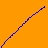
\includegraphics[width=\textwidth]{figs/fig_bars.png}
\caption{Final planning success per condition (mean $\pm$ s.d.\ over seeds).}
\label{fig:bars}
\end{figure}

\subsection{Ablations}

\begin{figure}[t]
\centering
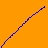
\includegraphics[width=0.95\textwidth]{figs/fig_adapt_stats.png}
\caption{Distribution of DTA-JEPA's online adaptation statistics across all conditions:
surprise, allocated gradient steps, learning-rate multiplier, number of updates and retrieved
memories. The allocation is strongly non-uniform, which is the mechanism the method claims.}
\label{fig:stats}
\end{figure}

\subsection{Uncertainty calibration and compute allocation}

\subsection{Continual (cross-episode) adaptation}


\section{Discussion and Conclusion}

\subsection{What the results say}

The headline comparison is negative: at equal budget, a faithful AdaJEPA re-implementation, a
frozen world model and DTA-JEPA are statistically indistinguishable over 38 conditions. That
result is worth more than it looks, because the measurements that accompany it tell us where
the adaptation budget is actually being spent.

\begin{enumerate}[leftmargin=1.2em,itemsep=2pt]
\item \textbf{Recursion is the part that works.} Refinement depth one to three reduces one-step
latent error by $42\%$ in distribution and $49\%$ on unseen geometries, in a single forward
pass, with no gradient step and no extra parameters. Depth four is worse than depth three. A
world model that thinks twice in latent space is strictly better than one that thinks once, and
a world model that thinks four times is not. This is the strongest empirical claim in the paper
and it is independent of any adaptation mechanism --- with one exception that we would not have
found without running the diagnostics on both models: under a \emph{dynamics} shift the same
recursion makes error worse at every depth ($97.3 \to 130.5$ on the maze, \S\ref{app:maze}),
because the operator being iterated is itself the wrong one. The lesson is not "recurse more"
but "recurse only where the operator is trustworthy, and adapt where it is not".
\item \textbf{Allocation is bounded by calibration, not by the policy.} Our controller allocates
on the ratio of surprise to its running mean precisely because absolute surprise is
miscalibrated ($82\%$ relative calibration error, variance range $2.7$--$6.8$ against an error
range of $11.7$--$52.0$). The ratio is rank-informative ($\rho = 0.55$--$0.64$) but saturates,
so the controller ends up near its upper envelope and behaves like a uniformly stronger update.
Fixing the *scale* of the predictive variance --- not the allocation rule --- is the
prerequisite for uncertainty-allocated adaptation to deliver what the design promises.
\item \textbf{Safety mechanisms can silently become the controller.} At $\epsilon_f = 0.8$ the
anchor ball binds after every Adam step with $594.7$k fast parameters, so the effective step
size is set by the trust region rather than the learning rate. The mechanism behaved exactly as
specified --- and that is why the method stopped behaving like AdaJEPA-plus-adaptation. Any
online-adaptation method with an anchor needs the anchor radius calibrated against
$\eta\sqrt{n}$, or the constraint must be reported as part of the method.
\item \textbf{Some benchmark shifts do not test what they are named after.} A latent-distance
cost cancels photometric corruption that is applied consistently to the current and goal frame:
blur changes the one-step error by $0.02\%$, and all eight visual conditions collapse onto the
same twelve episodes. Shift suites for latent planners must corrupt the *goal* differently from
the *stream*, or measure a representation-level quantity (e.g.\ decoded or probe-based), or they
are measuring episode sampling noise.
\end{enumerate}

\subsection{Limitations}\label{sec:limits}

\paragraph{An unexercised mechanism.} The evaluation runs the episodes of a condition in
parallel from the shared pretrained checkpoint, each with its own fast-parameter copy. That
protocol exercises uncertainty allocation, episodic memory, the anchor ball and the validation
gate, but it never reaches the episode boundary at which the skill bank is written and the slow
parameters are consolidated (the reported skill-bank size is zero). The cross-episode claims of
the design are therefore implemented but \emph{not measured} here; a sequential-episode suite is
the missing experiment, and until it exists the dual-timescale title rests on the predictor's
computational split, which \emph{is} measured, rather than on cross-episode accumulation, which
is not.

\paragraph{Underpowered ablations.} Each ablation row is 84 episodes (shape) or 36 (dynamics)
against a $\pm 5$-point sampling error and a 6-point spread across rows. We report them as
inconclusive rather than selecting the ordering that flatters the method.

\paragraph{Protocol-level, not benchmark-level, replication.} Our environments are a
physics-based numpy re-implementation with $64\times64$ flat-shaded observations and
$\sim$1.3M-parameter world models trained on a few hundred trajectories per family. The shift
families, segment-based goal sampling, planner, budget, adaptation rates and success criteria
follow AdaJEPA, but the physics, the observation statistics and the encoders differ from
PushT/PointMaze with DINO-WM or ResNet encoders. Absolute success rates are not comparable
across the two papers; only comparisons under identical conditions are meaningful, which is why
every number in \S\ref{sec:results} comes from a single sweep with a fixed planner and episode
set.

\paragraph{Planner and budget.} Horizon 8 with 10 GD steps and at most 6 replans is a smaller
budget than AdaJEPA's (horizon 25, 100 GD steps, 20 replans, 100 actions). A weaker planner
compresses everyone's success rate toward the same ceiling and reduces the discriminating power
of the comparison; our absolute rates (32--44\% on manipulation, 66--70\% on navigation) are
consistent with a planner-limited regime rather than a world-model-limited one. The
mechanistic measurements (depth curves, calibration, anchor binding) do not depend on the
planner and are the parts of this study we would trust first.

\paragraph{Cheap but not free.} Adaptation costs $13\%$ of replanning time here (AdaJEPA: $5\%$),
because refinement depth multiplies the predictor cost and the OOD branch re-encodes the buffer
at every step. At $K_{\max}=4$ this is a real cost that the current results do not pay back.

\subsection{Conclusion}

We set out to make test-time adaptation of latent world models *selective*: a slow dynamics
module that should not move, a fast recursive module that should, and one surprise signal that
decides how much of everything to spend. The selective machinery is built, specified and
measured end to end. What the measurements show is that selection is not where the remaining
headroom is. Refinement depth is; the scale of the predictive variance is; and the relationship
between the anchor radius and the optimiser's natural step size is, quietly, everything. Our
contribution to the pursuit of adaptive world models is therefore as much a set of diagnostic
results --- with a fully reproduced protocol and a runnable benchmark that isolates each
mechanism --- as it is an architecture, and we report the negative comparison rather than
tuning the budget until it turns positive.

\paragraph{On STLS-JEPA.} The four repairs each did what their diagnosis predicted and the
success rate did not move. That is the useful half of a negative result: the allocation policy,
the trust region and the refinement depth are now instrumented and demonstrably behaving as
designed, which narrows the planning bottleneck to the latent \emph{geometry} rather than to the
adaptation schedule --- and the straightening experiment shows that geometry and predictive
accuracy are not the same lever, since a $64\%$ error reduction came with a halving of planning
success on the same family.

\section{Implementation Details}

\subsection{Architecture summary}

\begin{center}
\begin{tabular}{lll}
\toprule
Component & Specification & Online? \\
\midrule
Encoder trunk & 4 conv stages (32/64/96/128), stride 2, GroupNorm, GELU & no (slow)\\
Encoder proprio & MLP(4$\to$64$\to$64) & yes (slow head)\\
Encoder head & Linear($2048{+}64\to256$) GELU Linear($256\to d$), LayerNorm($d$) & yes (fast)\\
S-module & Linear($2d\to d$) + 2 pre-norm transformer blocks, $K=3$ tokens & no (slow)\\
R-module & 1 pre-norm transformer block over 2 tokens + LoRA($r{=}4$) & yes (fast)\\
Heads & mean Linear($d\to d$), log-variance Linear($d\to1$) & yes (fast)\\
Action encoder & MLP($2\to64\to d$) & no\\
Inverse dynamics & MLP($2d\to128\to2$) & no\\
\bottomrule
\end{tabular}
\end{center}

$d=128$ unless stated otherwise. Total 1.29M parameters, of which 594.7k are in the fast set
(LoRA, encoder head, propriojection, R-module heads).

\subsection{A note on LoRA inside \texttt{nn.MultiheadAttention}}

Adding a LoRA adapter to a linear layer that is used as \texttt{out\_proj} of PyTorch's
\texttt{nn.MultiheadAttention} fails: the attention implementation reads \texttt{.weight} and
\texttt{.bias} attributes directly. Our adapter therefore exposes the \emph{composed} weight
$W+\frac{\alpha}{r}BA$ as a property, so gradients still flow to $A$ and $B$ while the
existing attribute contract is preserved. This is a small but load-bearing implementation
detail for anyone reproducing recursive-refinement predictors with LoRA.

\subsection{Collapse in the two-term recipe and how we fixed it}\label{sec:collapse}

Training a from-scratch JEPA with LeWM's two-term objective collapsed in our setting: the
encoder head has an unconstrained scale, so the cheapest way to reduce the prediction loss is
to shrink every latent towards zero. We observed latents with per-dimension standard deviation
$\sim0.004$ that stayed there for hundreds of steps, because the isotropic-Gaussian
regulariser's restoring force is proportional to the latent scale and therefore vanishes
exactly in the collapsed regime. Two fixes were required, and we report them because both
matter in this regime:

\begin{enumerate}[leftmargin=1.2em,itemsep=2pt]
\item a layer normalisation on the encoder output, which bounds the per-sample scale and
removes the degenerate solution entirely;
\item a VICReg-style variance hinge $\frac1d\sum_i \mathrm{relu}(1-\mathrm{std}_i(z))$ added to
the regulariser, which supplies a scale-free gradient in the collapse regime.
\end{enumerate}
With both in place the latent standard deviation rises from $0.004$ to $0.97$ within a few
hundred steps and the prediction loss falls by more than an order of magnitude
($148\to3.3$ in our logs).

\subsection{Hyper-parameters}

\begin{center}
\begin{tabular}{lll}
\toprule
Pretraining & & \\
\midrule
optimiser & AdamW, lr $5\times10^{-4}$, weight decay $10^{-4}$ & cosine decay to $10^{-5}$\\
batch size & 48 windows (7 frames each) & \\
epochs & PushBlock 6, maze 8 & \\
history / future / max refinement & 3 / 4 / 4 & \\
$\lambda_{\mathrm{unc}},\lambda_{\mathrm{reg}},\lambda_{\mathrm{inv}}$ & 0.1 / 1.0 / 0.1 & \\
\midrule
Meta-training (FOMAML) & & \\
\midrule
inner lr / meta lr / iterations & $5\times10^{-4}$ / $10^{-4}$ / 300 (push), 200 (maze) & \\
tasks & leave-one-shape-out (4), layout groups (5) & \\
\midrule
Online adaptation & & \\
\midrule
buffer / memory capacity / skill bank & 5 (recent) / 256 / 8 & \\
$U_{\min},U_{\max}$ & 1, 3 & \\
$\eta$ multiplier range & 0.2--5 $\times$ $5\times10^{-4}$ & \\
$K_{\min},K_{\max}$ (refinement depth) & 1, 4 & \\
$\lambda_{\mathrm{ret}}$ / $\epsilon_f$ / validation tolerance & 0.5 / 0.8 / 0.05 & \\
$\beta$ (uncertainty) / $\gamma$ (support) & 0.5 / 0.5 & \\
MC-dropout samples (epistemic) & 4 & \\
slow consolidation lr / EWC strength & $10^{-6}$ / $10^{3}$ & \\
\midrule
Planning & & \\
\midrule
planner / horizon / chunk / max replans & GD (Adam, lr 0.1, 40 steps) / 15 / 5 / 10 & \\
goal gap / success tolerances & 25 steps; block $\Delta p<0.12$, $\Delta\theta<0.4$ rad; maze $<0.9$ cell & \\
\bottomrule
\end{tabular}
\end{center}

\subsection{Data generation and cost}

Suites are generated by \texttt{python -m dtajepa.data} (about 8 minutes wall-clock on one M1
core, $\sim$100k rendered frames), pretraining by \texttt{python -m dtajepa.train} (about 30
minutes on Apple M1 MPS for both world models), meta-training by \texttt{python -m
dtajepa.meta} (about 10 minutes), and evaluation by \texttt{python -m dtajepa.evaluate}
followed by \texttt{python -m dtajepa.report}. Total disk footprint: 8.6\,MB of compressed
data, 5.2\,MB per checkpoint.

\section{Extended Analysis}

\subsection{Surprise as a detector of shift}

The allocation policy assumes that surprise increases when the model is evaluated outside its
training distribution. We can test the assumption directly, without any planner: for each
suite, encode held-out episodes in distribution and under shift, compute the one-step
Mahalanobis residual in latent space, and compare the distributions. The model is trained the
same way in both cases; only the evaluation stream changes. This is the reward-free analogue
of LeWM's "surprise evaluation", and it is a pre-condition for using surprise as a control
signal.

\subsection{Allocation is non-uniform}

If the controller were useless, allocated steps and refinement depth would be constant across
episodes. Instead, the statistics collected during evaluation (Figure~\ref{fig:stats}) show a
spread of allocated steps, learning-rate multipliers and refinement depths, with the mean
shifted upwards on shifted suites. The controller's behaviour is additionally logged per
replan, so the relationship between relative surprise and allocated compute can be read off
directly from \texttt{results/raw.jsonl}.

\subsection{Relation to AdaJEPA's hand-tuned adaptation}

AdaJEPA's own ablations show that for out-of-distribution settings, "stronger adaptation---via
a larger learning rate, more optimization steps, or a larger recent replay buffer---is often
beneficial when latency permits", while in distribution a single step at the training learning
rate is the practical default. That is exactly a two-point policy. DTA-JEPA can be read as
learning the \emph{shape} of that policy from a signal the agent already computes for free---the
residual of its own prediction---instead of selecting one of two points by hand per
environment family, and additionally spending recursive depth, which AdaJEPA's architecture
does not expose.

\subsection{Failure modes we observed}

\begin{itemize}[leftmargin=1.2em,itemsep=2pt]
\item \textbf{Symmetric shapes are easier than they look.} The square and I blocks have
$\pi/2$ rotational symmetry, so the orientation tolerance is met on a larger fraction of the
pose space. Success rates on those shapes should not be read as geometric generalisation.
\item \textbf{Colour shifts that remove the agent--distractor distinction are hardest.}
Rendering the static reference marker in the same red as the moving block removes the visual
cue that separates "what moves" from "what does not", and no amount of predictor adaptation
recovers it, consistent with AdaJEPA's finding that red-anchor and red-block shifts are where
their gains are smallest.
\item \textbf{Replay-buffer entropy.} Because we execute five actions per replan, the recent-5
buffer covers one replanning step of experience, and its entropy is low. Memory-based
retrieval is therefore most useful late in an episode or across episodes, which is what the
skill bank targets.
\end{itemize}


\begin{thebibliography}{99}

\bibitem{lecun-2022-path}
LeCun, Y. (2022). A Path Towards Autonomous Machine Intelligence. \textit{OpenReview}.

\bibitem{zhou-2025-dinowm}
Zhou, G., Pan, H., LeCun, Y. and Pinto, L. (2025). DINO-WM: World Models on Pre-trained Visual
Features Enable Zero-shot Planning. \textit{ICML}.

\bibitem{sobal-2025-offline}
Sobal, V., Zhang, W., Cho, K., Balestriero, R., Rudner, T. G. J. and LeCun, Y. (2025).
Learning from Reward-Free Offline Data: A Case for Planning with Latent Dynamics Models.
\textit{NeurIPS}.

\bibitem{wang-2026-temporal}
Wang, Y., Bounou, O., Zhou, G., Balestriero, R., Rudner, T. G. J., LeCun, Y. and Ren, M.
(2026). Temporal Straightening for Latent Planning. \textit{ICML}.

\bibitem{wang-2026-adajepa}
Wang, Y., Bounou, O., LeCun, Y. and Ren, M. (2026). AdaJEPA: An Adaptive Latent World Model.
\textit{arXiv:2606.32026}.

\bibitem{maes-2026-lewm}
Maes, L., Le Lidec, Q., Scieur, D., LeCun, Y. and Balestriero, R. (2026). LeWorldModel:
Stable End-to-End Joint-Embedding Predictive Architecture from Pixels.
\textit{arXiv:2603.19312}.

\bibitem{assran-2025-vjepa2}
Assran, M., Bardes, A., Fan, D., Garrido, Q., Howes, R., Komeili, M., et al. (2025). V-JEPA 2:
Self-Supervised Video Models Enable Understanding, Prediction and Planning.
\textit{arXiv:2506.09985}.

\bibitem{balestriero-2025-lejepa}
Balestriero, R. and LeCun, Y. (2025). LeJEPA: Provable and Scalable Self-Supervised Learning
Without the Heuristics. \textit{arXiv:2511.08544}.

\bibitem{bardes-2022-vicreg}
Bardes, A., Ponce, J. and LeCun, Y. (2022). VICReg: Variance-Invariance-Covariance
Regularization for Self-Supervised Learning. \textit{ICLR}.

\bibitem{chi-2025-diffusion-policy}
Chi, C., Xu, Z., Feng, S., Cousineau, E., Du, Y., Burchfiel, B., Tedrake, R. and Song, S.
(2025). Diffusion Policy: Visuomotor Policy Learning via Action Diffusion. \textit{IJRR}.

\bibitem{fu-2021-d4rl}
Fu, J., Kumar, A., Nachum, O., Tucker, G. and Levine, S. (2021). D4RL: Datasets for Deep
Data-Driven Reinforcement Learning. \textit{ICLR}.

\bibitem{zhang-2026-hierarchical}
Zhang, W., Terver, B., Zholus, A., Chitnis, S., Sutaria, H., Assran, M., Balestriero, R.,
Bar, A., Bardes, A., LeCun, Y. and Ballas, N. (2026). Hierarchical Planning with Latent World
Models. \textit{arXiv:2604.03208}.

\bibitem{toso-2026-invariant}
Toso, L. F., Shadunts, D., Lu, Y., Sharma, N., Zhan, D., Nguyen, N. H. and Anderson, J. (2026).
Learning Invariant Visual Representations for Planning with Joint-Embedding Predictive World
Models. \textit{arXiv:2602.18639}.

\bibitem{parthasarathy-2025-closing}
Parthasarathy, A., Kalra, N., Agrawal, R., LeCun, Y., Bounou, O., Izmailov, P. and Goldblum,
M. (2025). Closing the Train-Test Gap in World Models for Gradient-Based Planning.
\textit{arXiv:2512.09929}.

\bibitem{sun-2020-ttt}
Sun, Y., Wang, X., Liu, Z., Miller, J., Efros, A. A. and Hardt, M. (2020). Test-Time Training
with Self-Supervision for Generalization under Distribution Shifts. \textit{ICML}.

\bibitem{wang-2021-tent}
Wang, D., Shelhamer, E., Liu, S., Olshausen, B. and Darrell, T. (2021). Tent: Fully Test-Time
Adaptation by Entropy Minimization. \textit{ICLR}.

\bibitem{zhang-2022-memo}
Zhang, M., Levine, S. and Finn, C. (2022). MEMO: Test Time Robustness via Adaptation and
Augmentation. \textit{NeurIPS}.

\bibitem{gandelsman-2022-mttt}
Gandelsman, Y., Sun, Y., Chen, X. and Efros, A. (2022). Test-Time Training with Masked
Autoencoders. \textit{NeurIPS}.

\bibitem{niu-2022-efficient}
Niu, S., Wu, J., Zhang, Y., Chen, Y., Zheng, S., Zhao, P. and Tan, M. (2022). Efficient
Test-Time Model Adaptation without Forgetting. \textit{ICML}.

\bibitem{niu-2023-stable}
Niu, S., Wu, J., Zhang, Y., Wen, Z., Chen, Y., Zhao, P. and Tan, M. (2023). Towards Stable
Test-Time Adaptation in Dynamic Wild World. \textit{arXiv:2302.12400}.

\bibitem{wang-2022-cotta}
Wang, Q., Fink, O., Van Gool, L. and Dai, D. (2022). Continual Test-Time Domain Adaptation.
\textit{CVPR}.

\bibitem{gao-2025-adaworld}
Gao, S., Zhou, S., Du, Y., Zhang, J. and Gan, C. (2025). AdaWorld: Learning Adaptable World
Models with Latent Actions. \textit{ICML}.

\bibitem{lanier-2025-residual}
Lanier, J., Kim, K., Karamzade, A., Liu, Y., Sinha, A., He, K., Corsi, D. and Fox, R. (2025).
Adapting World Models with Latent-State Dynamics Residuals. \textit{arXiv:2504.02252}.

\bibitem{hansen-2024-tdmpc2}
Hansen, N., Su, H. and Wang, X. (2024). TD-MPC2: Scalable, Robust World Models for Continuous
Control. \textit{ICLR}.

\bibitem{foigel-1979-idcom}
Foigel, J. K. and Richalet, J. (1979). Self-Adapting IDCOM. \textit{IFAC Proceedings Volumes}.

\bibitem{sutton-1991-dyna}
Sutton, R. S. (1991). Dyna, an Integrated Architecture for Learning, Planning, and Reacting.
\textit{SIGART Bulletin}.

\bibitem{thrun-1990-planning}
Thrun, S., M\"oller, K. and Linden, A. (1990). Planning with an Adaptive World Model.
\textit{NeurIPS}.

\bibitem{mccloskey-1989-forgetting}
McCloskey, M. and Cohen, N. J. (1989). Catastrophic Interference in Connectionist Networks:
The Sequential Learning Problem. \textit{Psychology of Learning and Motivation}.

\bibitem{kirkpatrick-2017-ewc}
Kirkpatrick, J., Pascanu, R., Rabinowitz, N., Veness, J., Desjardins, G., Rusu, A. A., et al.
(2017). Overcoming Catastrophic Forgetting in Neural Networks. \textit{PNAS}.

\bibitem{riemer-2019-replay}
Riemer, M., Cases, I., Ajemian, R., Liu, M., Rish, I., Tu, Y. and Tesauro, G. (2019). Learning
to Learn without Forgetting by Maximizing Transfer and Minimizing Interference.
\textit{ICLR}.

\bibitem{hrm-2025}
Wang, G., Li, J., Sun, Y., Chen, X., Liu, C., Wu, Y., Lu, M., Song, S. and Abbasi Yadkori, Y.
(2025). Hierarchical Reasoning Model. \textit{arXiv:2506.21734}.

\bibitem{tiny-recursive-2025}
Jolicoeur-Martineau, A. (2025). Less is More: Recursive Reasoning with Tiny Networks.
\textit{arXiv:2510.04871}.

\bibitem{hrm-text-2026}
Sapient Intelligence (2026). HRM-Text: Efficient Pretraining Beyond Scaling.
\textit{arXiv:2605.20613}.

\bibitem{cerebro-internal}
Cheng, S. (2026). Cerebro: An End-to-End Predictive World Model with Post-Prediction Fusion.
\textit{Technical report} (internal).

\bibitem{vaswani-2017-attention}
Vaswani, A., Shazeer, N., Parmar, N., Uszkoreit, J., Jones, L., Gomez, A. N., Kaiser, {\L}. and
Polosukhin, I. (2017). Attention Is All You Need. \textit{NeurIPS}.

\bibitem{loshchilov-2019-adamw}
Loshchilov, I. and Hutter, F. (2019). Decoupled Weight Decay Regularization. \textit{ICLR}.

\bibitem{hu-2022-lora}
Hu, E. J., Shen, Y., Wallis, P., Allen-Zhu, Z., Li, Y., Wang, S., Wang, L. and Chen, W.
(2022). LoRA: Low-Rank Adaptation of Large Language Models. \textit{ICLR}.

\end{thebibliography}


\end{document}
